\documentclass{article}

% ==========================================
%           PACKAGES & DEFINITIONS
% ==========================================
\usepackage[utf8]{inputenc}
\usepackage[T1]{fontenc}
\usepackage{fancyhdr}
\usepackage{xcolor}
\usepackage[top=2.5cm,bottom=2.5cm, left=2.5cm, right=2.5cm]{geometry}
\usepackage{titlesec}
\usepackage{enumitem}
\usepackage{hyperref}
\usepackage{graphicx}
\usepackage{wrapfig}
\usepackage{setspace}
\usepackage{tabularx}
\usepackage{booktabs}
\usepackage{makecell}
\usepackage{changepage}
\usepackage{float}
\usepackage{microtype}
\usepackage{tcolorbox}
\usepackage{listings}
\tcbuselibrary{listings,breakable}

% --- Colors ---
\definecolor{dominantColor}{HTML}{000000}

% --- Section Formatting ---
\titleformat{\section}
{\color{dominantColor}\fontsize{22}{2.2em}\selectfont\bfseries}
{\thesection.}{0.3em}{}

\titleformat{\subsection}
{\color{dominantColor}\fontsize{18}{2.2em}\selectfont\bfseries}
{\thesubsection.}{0.3em}{}

% --- Header / Footer ---
\newcommand{\makeHeaderFooter}{
\thispagestyle{fancy}
\fancyhead{}
\rhead{
\includegraphics[width=3cm]{pics/esi.png}}
\lhead{
\includegraphics[width=4cm]{pics/project_logo.jpg}}
\renewcommand{\headrulewidth}{0pt}
\fancyfoot{}
\cfoot{\fontsize{12pt}{1.2em}{\textbf{1 May 2026}}}
}

\hypersetup{
colorlinks,
linkcolor=black,
urlcolor=black
}

\setlength{\parindent}{0pt}
\setlength{\parskip}{1.2em}
\onehalfspacing

% --------------------------
% Python code style box
% --------------------------
\newtcblisting{pythoncode}[1][]{
    listing engine=listings,
    colback=black!95!white,
    colframe=black,
    coltitle=white,
    listing only,
    breakable,
    enhanced,
    sharp corners,
    boxrule=0.5mm,
    top=2mm, bottom=2mm, left=2mm, right=2mm,
    fonttitle=\bfseries,
    title=#1,
    listing options={
        language=Python,
        basicstyle=\ttfamily\footnotesize\color{white},
        keywordstyle=\color{cyan},
        commentstyle=\color{green!70!black},
        stringstyle=\color{orange},
        showstringspaces=false,
        breaklines=true
    }
}

% ==========================================
%               DOCUMENT
% ==========================================
\begin{document}

% ==========================================
%               TITLE PAGE
% ==========================================
\begin{titlepage}
\vspace*{\fill}

{\color{dominantColor}\hrule}
\vspace{0.6cm}

\begin{center}
\fontsize{40pt}{1.2em}\selectfont\textbf{Project Report}
\end{center}

\vspace{0.6cm}
{\color{dominantColor}\hrule}
\vspace{0.8cm}

\begin{center}
\fontsize{21pt}{1.4em}\selectfont
\textbf{Theme: Medical Prescription OCR with TrOCR}
\end{center}

\vspace{0.6in}

\begin{center}
\fontsize{19pt}{1.4em}\selectfont
This project tackles the long-standing problem of digitizing handwritten medical prescriptions by fine-tuning a Transformer-based vision encoder--decoder (TrOCR) and exposing it through a production-ready API and web interface.
\end{center}

\vspace{0.6in}

\begin{center}
\fontsize{17pt}{1.35em}\selectfont
\textbf{Group Members:} \\[0.3cm]
Benhammadi Lokmane \\[0.3cm]
Khedim Youcef \\[0.3cm]

% Add additional team members here
\end{center}

\vspace*{\fill}
\makeHeaderFooter
\end{titlepage}

% ==========================================
%               CONTENT
% ==========================================
\newpage
\pagestyle{fancy}
\fancyhf{}
\fancyhead[L]{Project Report}
\fancyhead[R]{\thepage}

\tableofcontents
\newpage
\listoffigures
\newpage

% ==========================================
%               SECTIONS
% ==========================================

\section{Introduction and Problem Statement}
\label{sec:intro}

\subsection{The Challenge: Reading Handwritten Medical Prescriptions}
Handwritten medical prescriptions remain one of the most stubborn last-mile problems in healthcare digitization. Despite the rise of electronic health records, a large share of prescriptions issued worldwide are still written by hand, often hastily, on small slips of paper. Misreadings at the pharmacy directly translate into dispensing errors, drug interactions, and patient harm.

Two challenges sit at the core of this project:
\begin{itemize}[noitemsep, topsep=0pt]
    \item \textbf{Recognition:} Doctors' handwriting is famously irregular --- abbreviations, overlapping strokes, and inconsistent spacing make it hostile to off-the-shelf OCR.
    \item \textbf{Structure:} Even after raw text is extracted, downstream systems need structured fields (drug name, dosage, frequency) rather than a free-text blob.
\end{itemize}

The central question is: \textit{``Can a fine-tuned vision--language model transcribe handwritten prescription lines accurately enough to be useful in a real digitization pipeline?''}

\subsection{Why Prescription OCR is Hard}
Three properties make prescriptions harder than typical handwritten text:
\begin{enumerate}[noitemsep, topsep=0pt]
    \item \textbf{Domain-specific vocabulary} --- drug names rarely occur in general handwriting corpora.
    \item \textbf{Layout variability} --- header letterhead, table-like dosage grids, and free-form notes mix in a single image.
    \item \textbf{Acquisition noise} --- prescriptions are typically captured with phone cameras, introducing skew, shadows, and uneven lighting.
\end{enumerate}

\subsection{Our Approach: Fine-Tuned Vision Encoder--Decoder}
We fine-tune Microsoft's \texttt{trocr-base-handwritten} on a public prescription dataset, wrap it in an end-to-end pipeline (preprocessing $\rightarrow$ line segmentation $\rightarrow$ TrOCR $\rightarrow$ post-processing), and expose it through a FastAPI backend and a React+Vite frontend.

\begin{figure}[H]
\centering
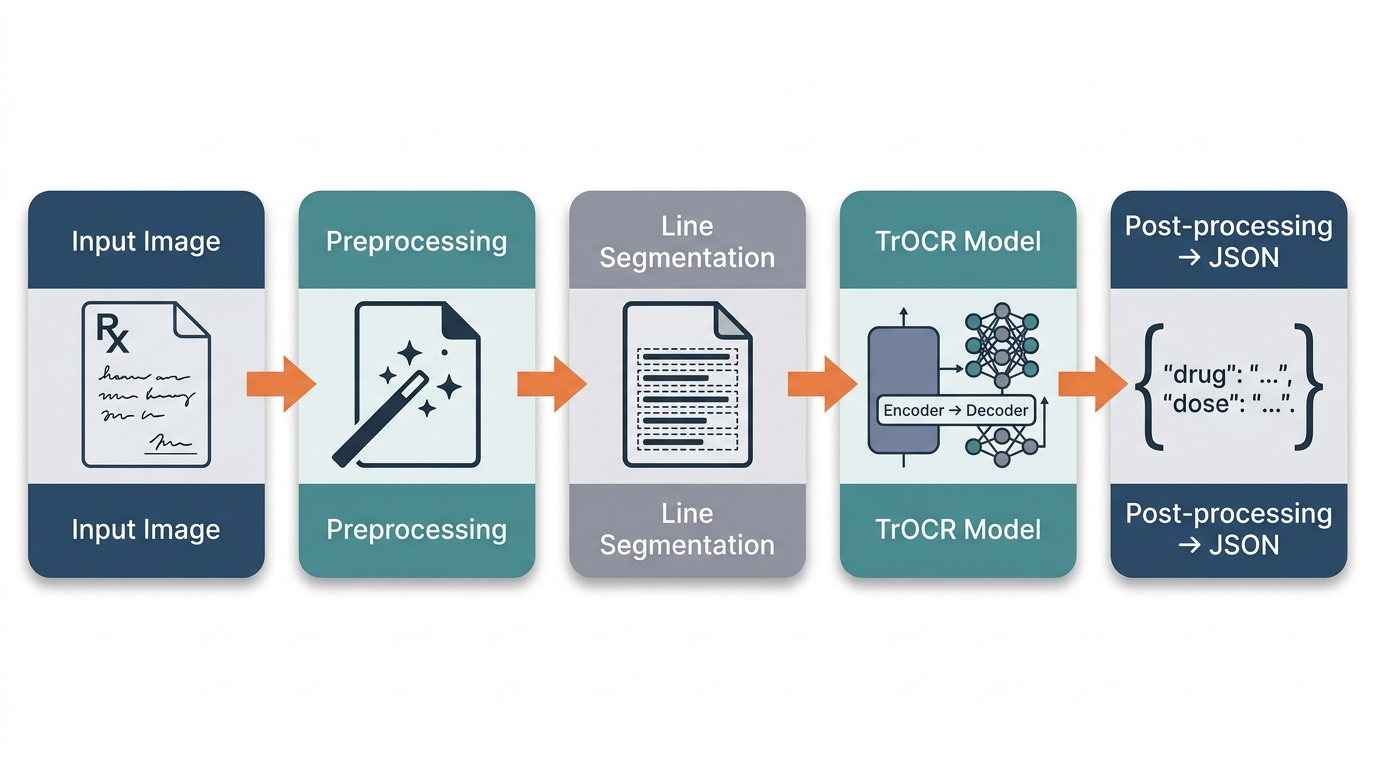
\includegraphics[width=1\textwidth]{pics/pipeline.png}
\caption{End-to-end medical prescription OCR pipeline.}
\label{fig:pipeline}
\end{figure}

\clearpage
\newpage

\section{Background: OCR and Vision Encoders}
\label{sec:background}

\subsection{From Classical OCR to Deep Learning}
Classical OCR engines (Tesseract, ABBYY) rely on hand-crafted features and per-character segmentation. They work well on clean printed text but break down on cursive handwriting, where character boundaries are ambiguous. The first deep-learning wave used CNN+RNN+CTC models (e.g.\ CRNN), which jumped accuracy on scene text but still struggled with long-range context in handwriting.

\subsection{The Vision Transformer (ViT)}
The Vision Transformer reframed image understanding as a sequence-modeling problem: an image is split into fixed-size patches (e.g.\ $16\times16$), each patch is linearly projected into an embedding, positional embeddings are added, and the resulting sequence is fed through a stack of self-attention layers --- exactly the architecture used in language Transformers.

\begin{figure}[H]
\centering
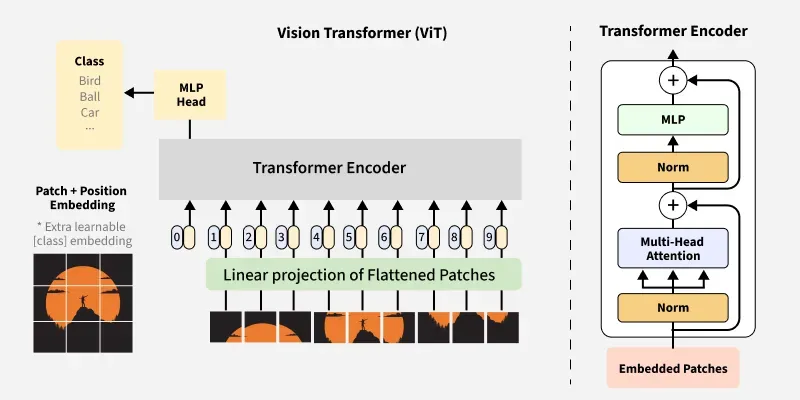
\includegraphics[width=0.8\textwidth]{pics/vit_architecture.png}
\caption{Vision Transformer (ViT): an image is split into patches and processed as a sequence.}
\label{fig:vit}
\end{figure}

\subsection{Encoder--Decoder Architectures for Image-to-Text}
For OCR, we need not just an image representation but a text generator. The encoder--decoder paradigm fits naturally: the encoder produces a sequence of visual tokens, and an autoregressive decoder generates output tokens one at a time, attending back to the encoder via cross-attention. This is the recipe behind TrOCR, Donut, and most modern document-AI models.

\clearpage
\newpage

\section{TrOCR: Model Architecture}
\label{sec:trocr}

\subsection{Overview of TrOCR}
TrOCR (\textit{Transformer-based Optical Character Recognition}, Li et al.\ 2021) is a fully Transformer-based encoder--decoder model. It pairs a pretrained image Transformer encoder (BEiT, ViT, or DeiT) with a pretrained text Transformer decoder (RoBERTa or similar). End-to-end fine-tuning then aligns the two for the OCR task.

% IMAGE: TrOCR architecture diagram (image encoder + text decoder + cross-attention)
% Source: Figure 1 of the TrOCR paper (Li et al. 2021, arXiv:2109.10282), or
%         redraw using the Microsoft TrOCR repo's diagram for clarity.
\begin{figure}[H]
\centering
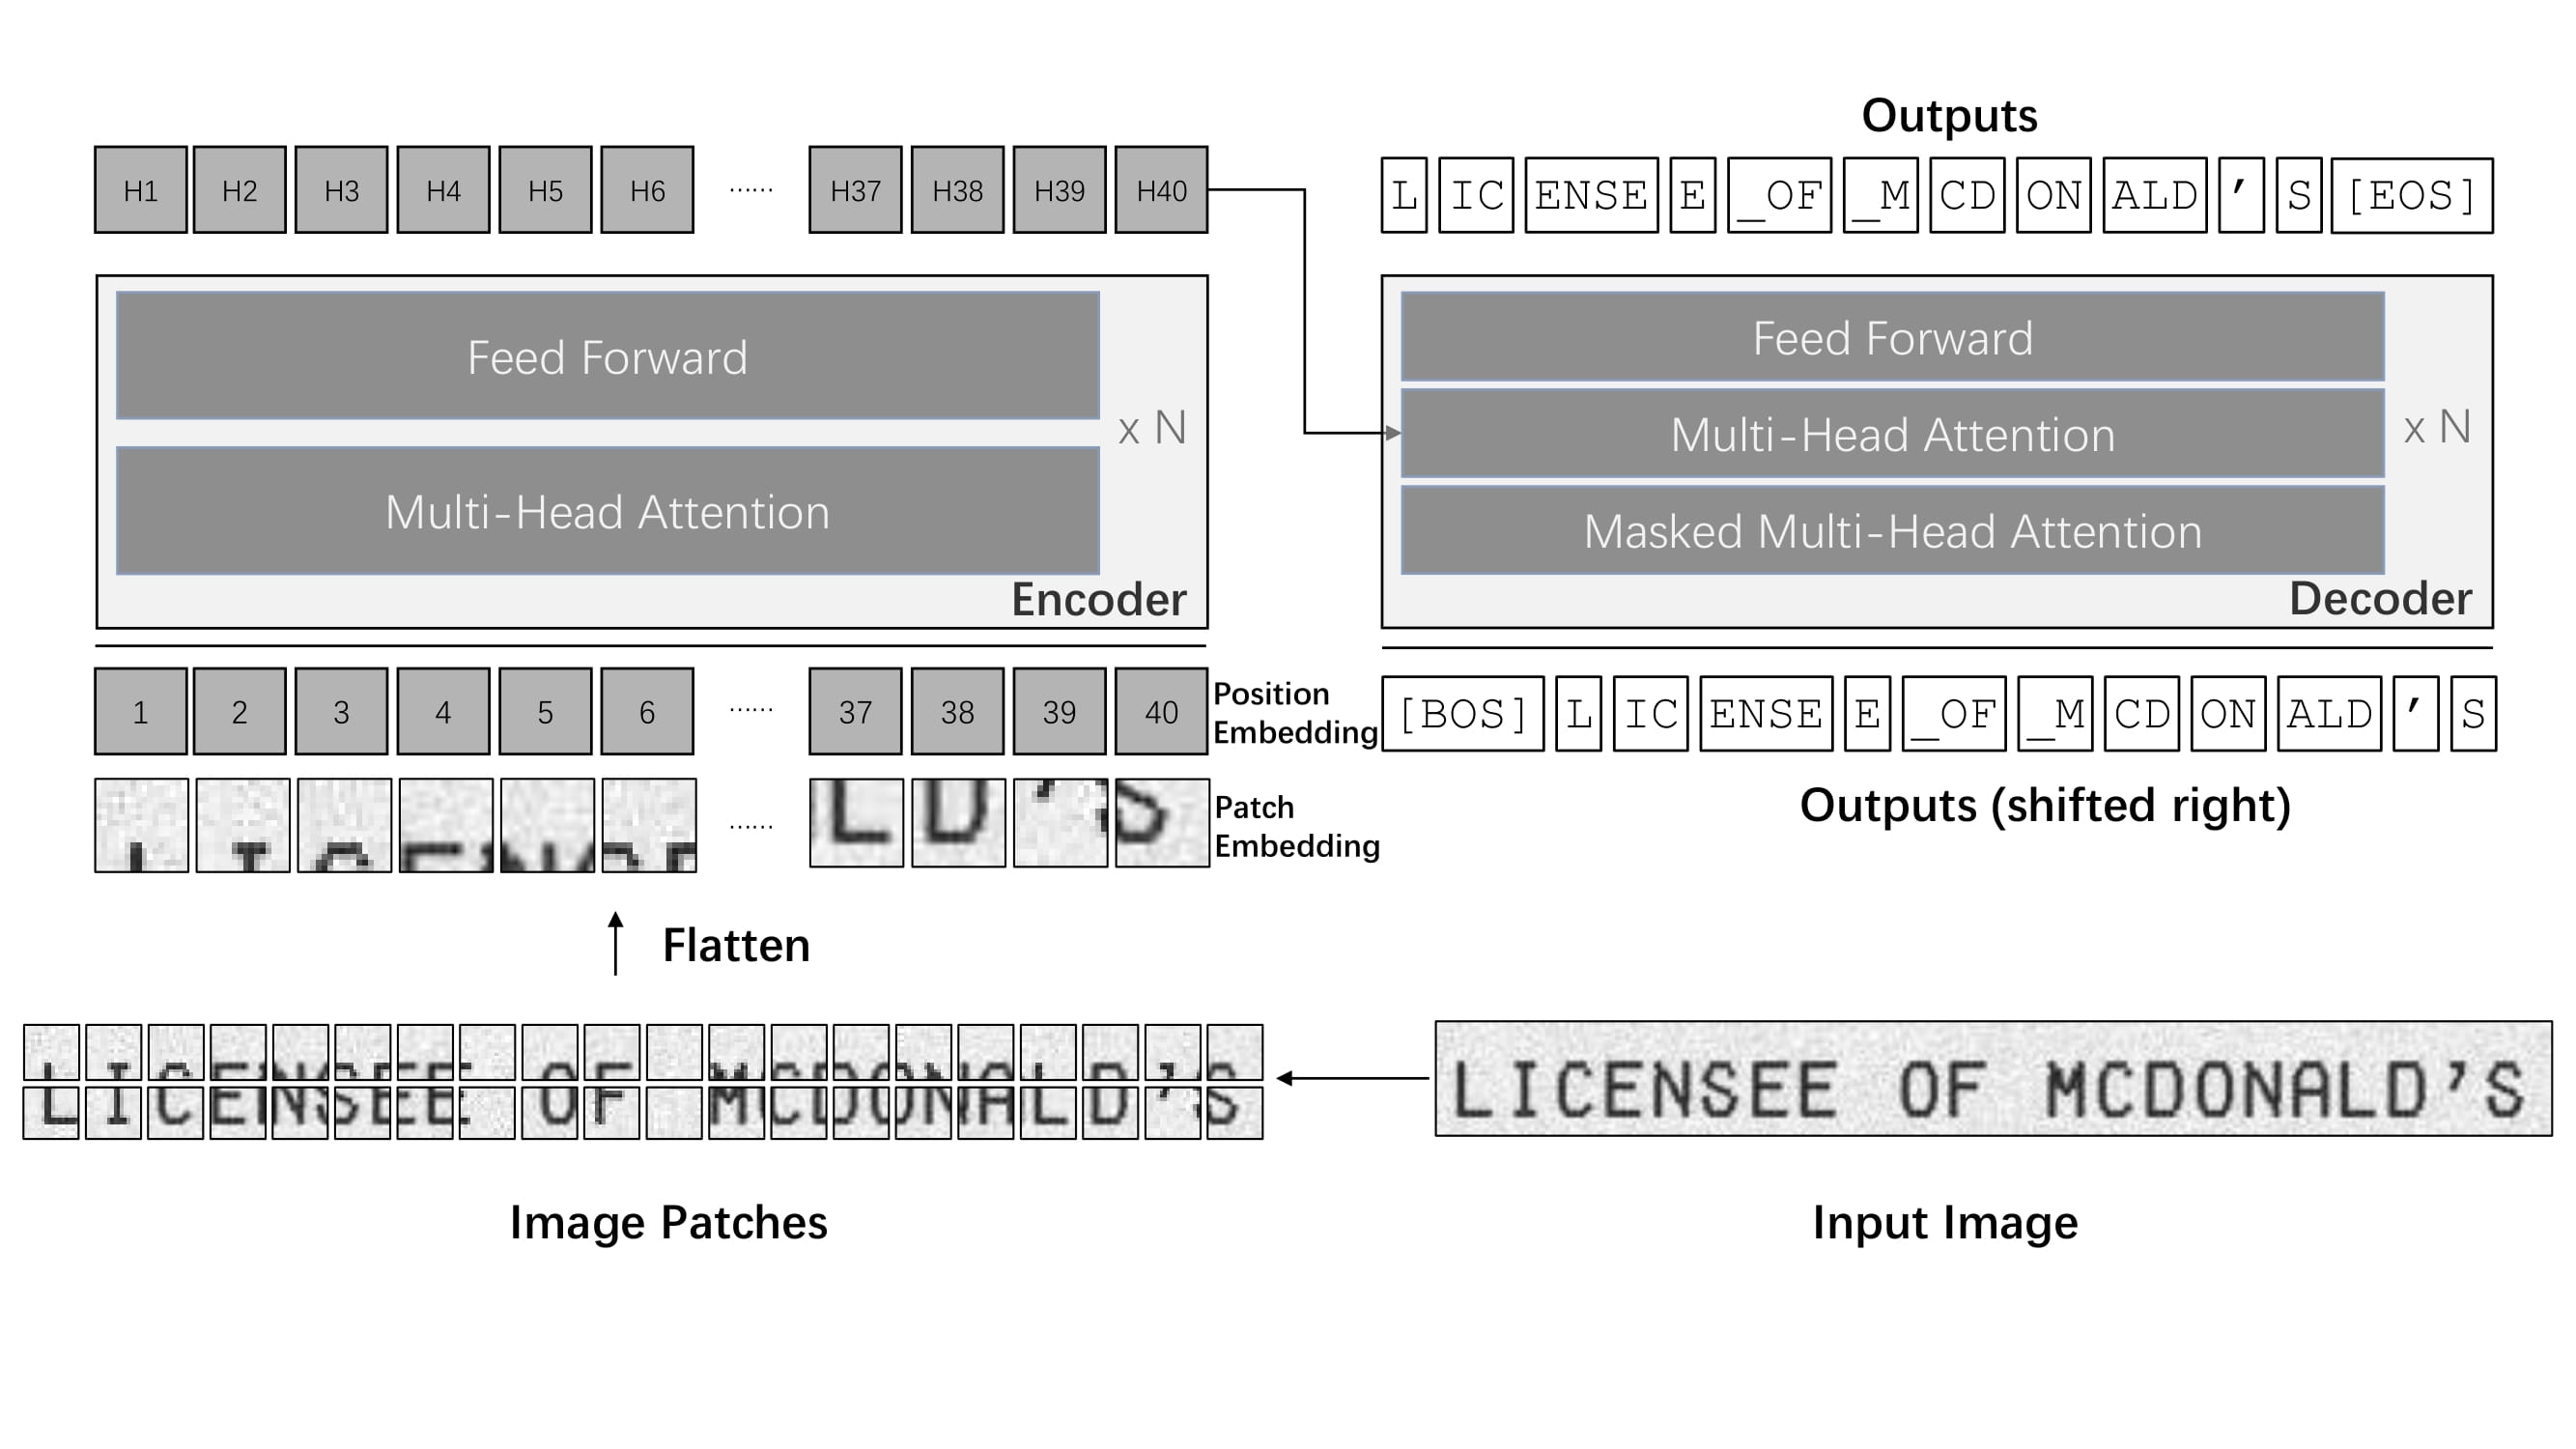
\includegraphics[width=0.95\textwidth]{pics/trocr_architecture.jpg}
\caption{TrOCR: a pretrained image Transformer encoder feeds a pretrained text Transformer decoder.}
\label{fig:trocr_arch}
\end{figure}

\subsection{The Image Encoder}
For \texttt{trocr-base-handwritten} the encoder is a BEiT-base model: 12 layers, hidden size 768, $384\times384$ input resized into $16\times16$ patches (576 patch tokens + 1 [CLS]). The encoder turns the image into a sequence of visual context vectors.

\subsection{The Text Decoder}
The decoder is a RoBERTa-style Transformer. At each step it consumes previously generated tokens (teacher-forced during training, autoregressive at inference) and attends to the encoder output through cross-attention to produce the next token.

\subsection{Cross-Attention and Generation}
Cross-attention is the bridge: decoder query vectors attend to encoder key/value vectors, letting each generated token ``look at'' the relevant region of the image. At inference we use beam search (beam size 2 in our config) to balance accuracy and latency.

\subsection{Why TrOCR for Handwritten Prescriptions}
Three reasons:
\begin{itemize}[noitemsep, topsep=0pt]
    \item It comes with a \textit{handwritten} variant pretrained on IAM, providing a strong starting point for cursive text.
    \item Its decoder has a real language model prior --- helpful for resolving ambiguous strokes using context.
    \item It plays nicely with HuggingFace tooling, making fine-tuning, checkpointing, and serving straightforward.
\end{itemize}

\clearpage
\newpage

\section{Dataset}
\label{sec:dataset}

\subsection{Source}
We use \texttt{chinmays18/medical-prescription-dataset} from the HuggingFace Hub: cropped line-level images of handwritten prescription text paired with ground-truth transcriptions.

\begin{figure}[H]
\centering
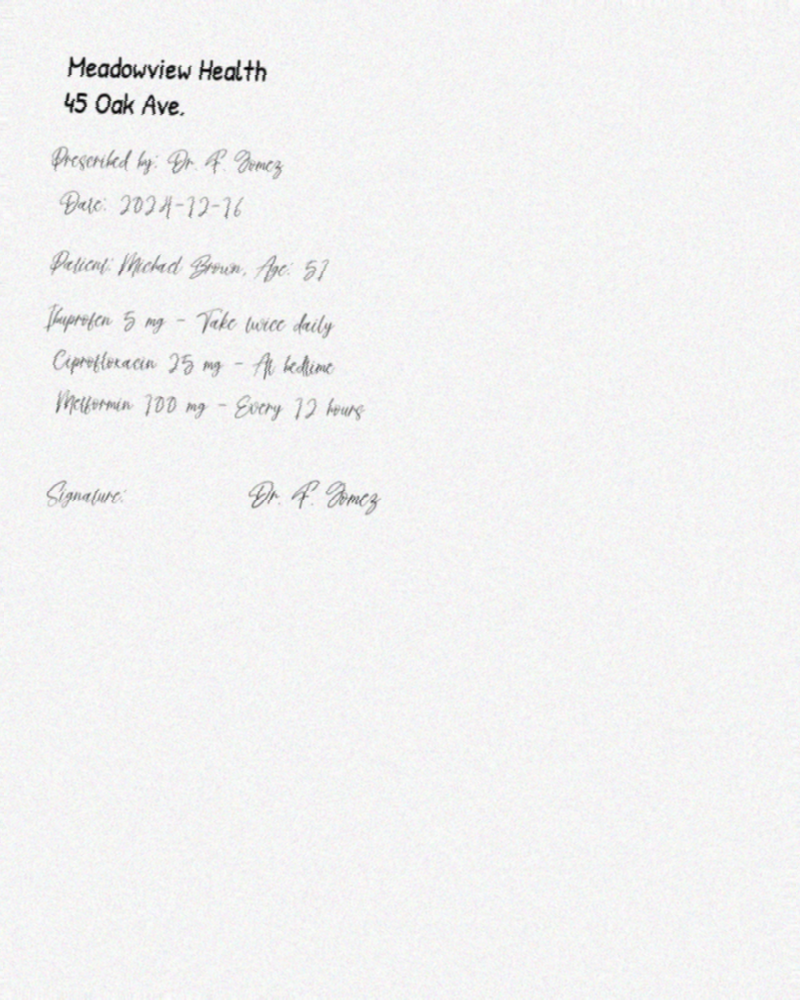
\includegraphics[width=0.55\textwidth]{pics/prescription_00000.png}
\caption{Examples from the prescription dataset: cropped lines with ground-truth labels.}
\label{fig:dataset_samples}
\end{figure}

The dataset annotations are structured to facilitate extraction of key clinical entities. Below is a sample of the ground-truth format used for training:

\begin{lstlisting}[language=json, breaklines=true, basicstyle=\small\ttfamily]
{
    "ground_truth": "<s_ocr> doctor_name: Dr. F. Gomez clinic_name: Meadowview Health clinic_address: 45 Oak Ave. patient_name: Michael Brown patient_age: 51 date: 2024-12-16 medications: - Ibuprofen 5 mg - Take twice daily - Ciprofloxacin 25 mg - At bedtime - Metformin 100 mg - Every 12 hours signature: Dr. F. Gomez </s>"
}
\end{lstlisting}

\subsection{Dataset Statistics}
% TABLE: replace these numbers with your actual dataset stats once you've inspected the splits

\begin{figure}[H]
\centering
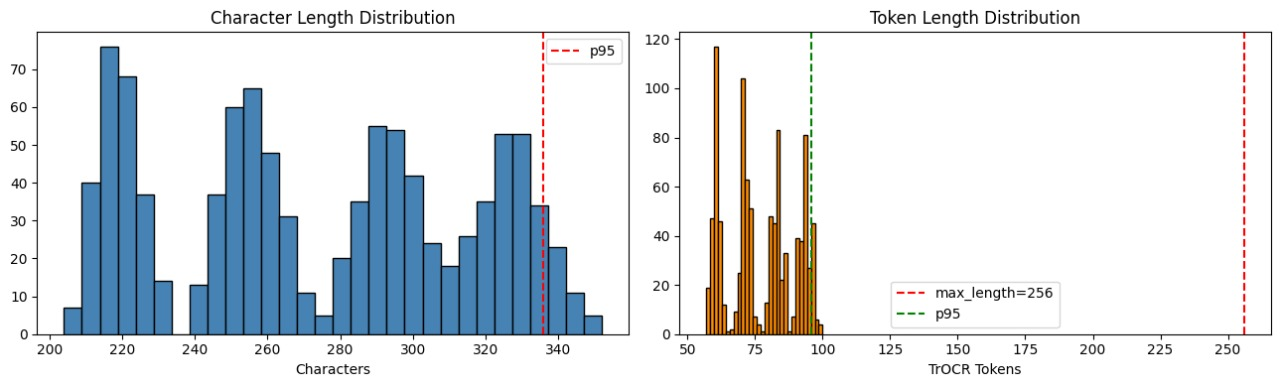
\includegraphics[width=\textwidth]{pics/chars_statistics.jpeg}
\caption{Distribution of character lengths (left) and token lengths (right) across the prescription dataset. The 95th percentile is highlighted in both plots to inform sequence length limits.}
\label{fig:char_token_stats}
\end{figure}

\begin{figure}[H]
\centering
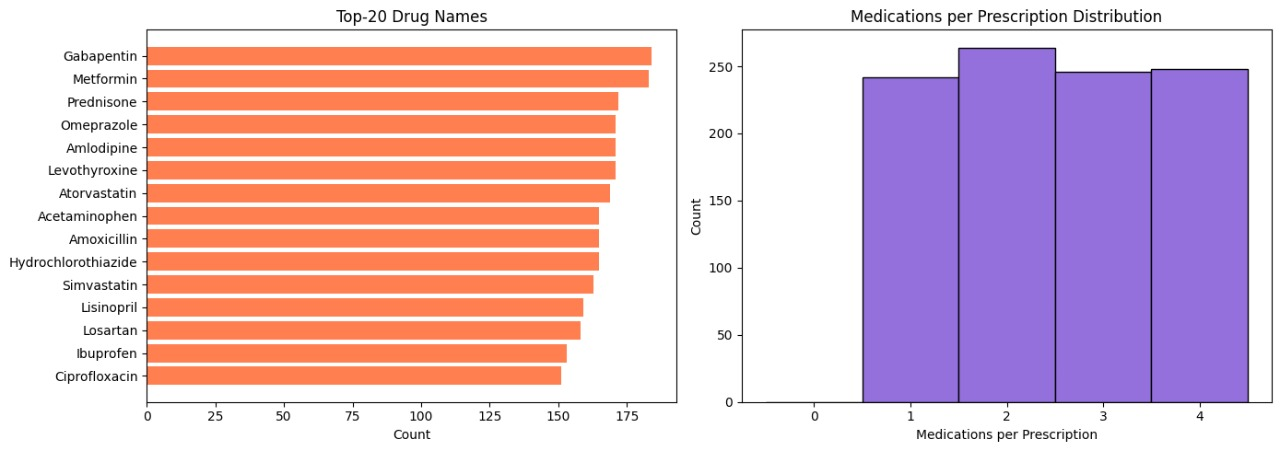
\includegraphics[width=\textwidth]{pics/drugs_statstics.jpg}
\caption{Frequency of the top-20 most commonly prescribed medications (left) and the distribution of the number of medications per prescription (right).}
\label{fig:drug_stats}
\end{figure}

\begin{figure}[H]
\centering
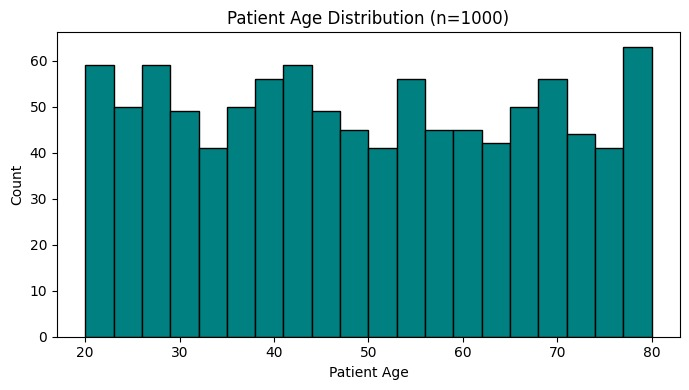
\includegraphics[width=0.7\textwidth]{pics/patient_ages.jpeg}
\caption{Age distribution of patients represented in the dataset ($n=1000$).}
\label{fig:age_stats}
\end{figure}

\subsection{Train / Validation / Test Split}
The split is controlled by \texttt{configs/config.yaml}: 80\% train, 10\% validation, 10\% test. Splits are seeded for reproducibility.

\clearpage
\newpage

\section{Preprocessing and Line Segmentation}
\label{sec:preprocessing}

\subsection{Image Cleanup}
Before TrOCR sees a crop, the raw photograph passes through a cleanup stage in \texttt{src/preprocess.py}: grayscale conversion, denoising, adaptive binarization, and deskewing.

% IMAGE: Before/after preprocessing — raw phone photo on the left, cleaned binarized version on the right
% Source: pick a sample from your test set, run it through src/preprocess.py, save both versions
\begin{figure}[H]
\centering
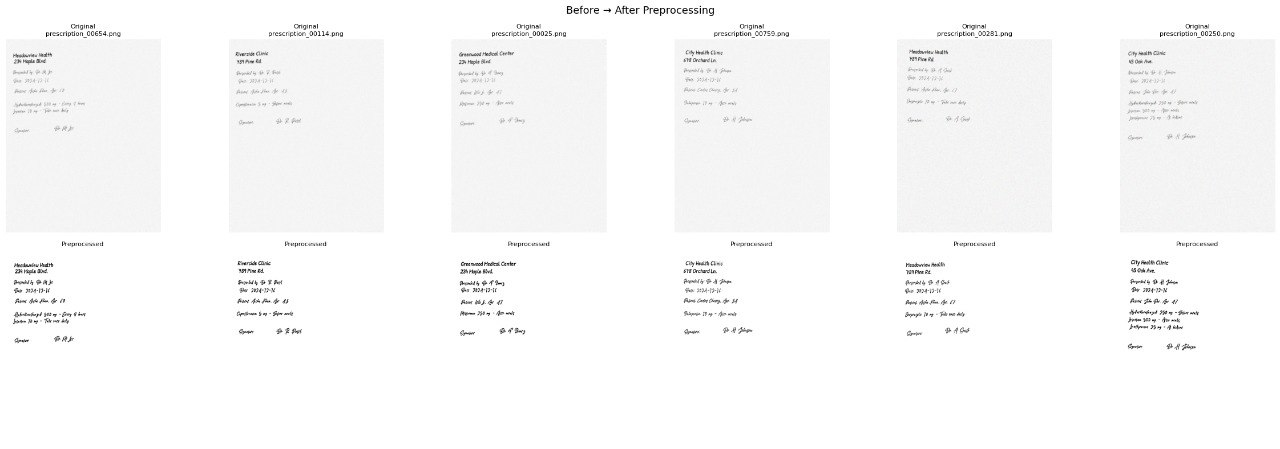
\includegraphics[width=0.8\textwidth]{pics/processing_images.jpg}
\caption{Effect of the preprocessing stage on a noisy phone-captured prescription.}
\label{fig:preprocess}
\end{figure}

\subsection{Line / Region Detection}
\texttt{src/detection/detector.py} segments the cleaned image into individual text lines using horizontal projection profiles followed by contour-based refinement. Each detected line is cropped and passed independently to TrOCR.

% IMAGE: Segmentation visualization — full prescription with detected line bounding boxes overlaid
% Source: instrument detector.py to draw rectangles around detected lines, save the result
\begin{figure}[H]
\centering
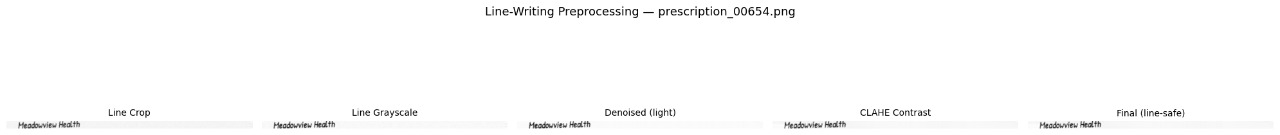
\includegraphics[width=0.85\textwidth]{pics/line_detction.jpg}
\caption{Detected line regions overlaid on the input prescription.}
\label{fig:segmentation}
\end{figure}

\subsection{TrOCR Processor}
\texttt{TrOCRProcessor} wraps the image processor (resize to $384\times384$, normalize with ImageNet statistics) and the tokenizer. The same processor is used at training and inference --- the artifact is loaded from the fine-tuned checkpoint to guarantee consistency.

\clearpage
\newpage

\section{Training Methodology}
\label{sec:training}

\subsection{Configuration}
All training settings live in \texttt{configs/config.yaml} so the same file drives training, evaluation, and inference. Key entries:

\begin{pythoncode}[configs/config.yaml]
model:
  name: "microsoft/trocr-base-handwritten"
  max_length: 128

training:
  epochs: 30
  batch_size: 8
  learning_rate: 5e-5
  weight_decay: 0.01
  warmup_steps: 500
  grad_clip: 1.0
  val_interval: 1
  checkpoint_dir: "checkpoints/"

inference:
  beam_size: 2
  device: "auto"
\end{pythoncode}

\subsection{Hardware: Kaggle 2$\times$T4 Setup}
Fine-tuning runs on a Kaggle notebook with two T4 GPUs (16~GB each). The notebook automates dataset download, training, evaluation, and pushing the final checkpoint to the HuggingFace Hub.

\begin{figure}[H]
\centering
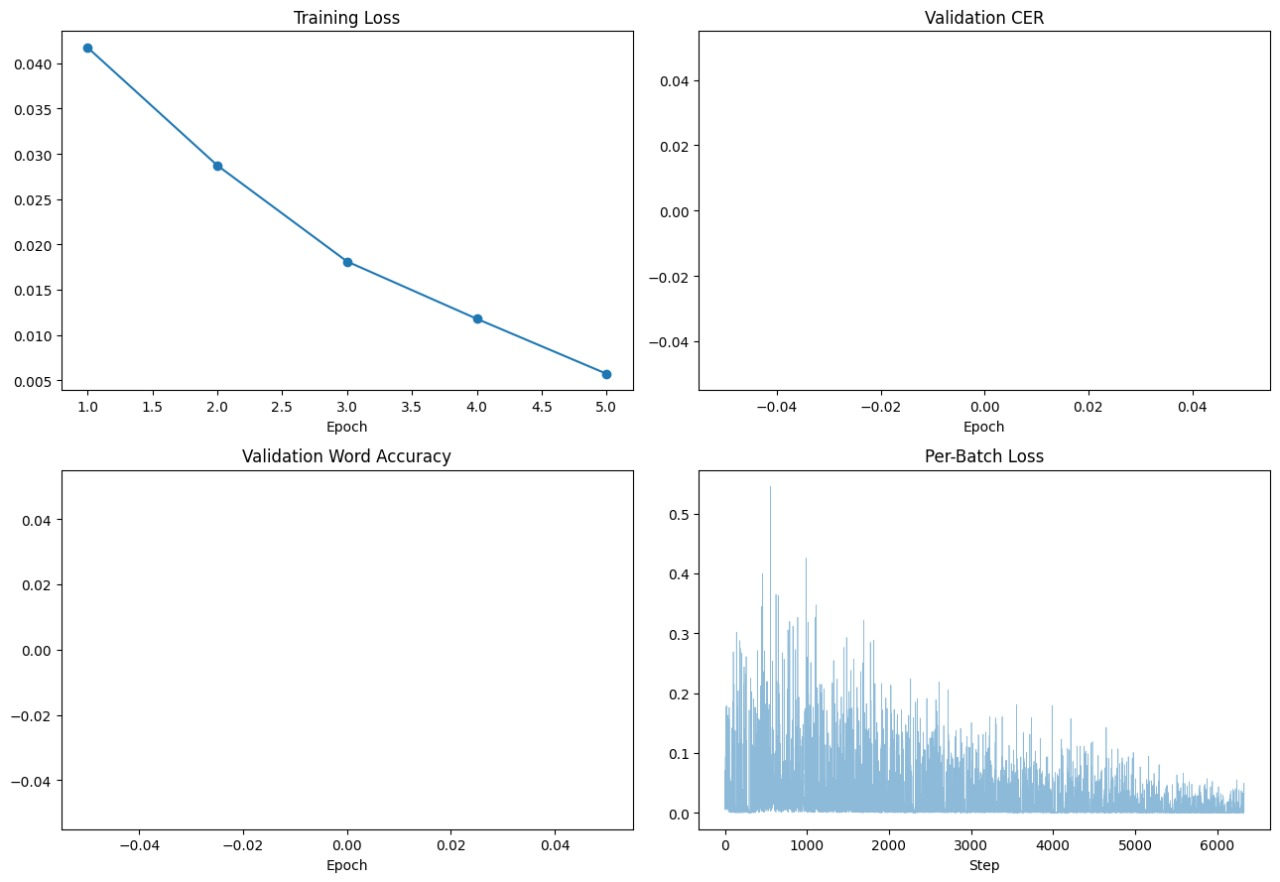
\includegraphics[width=\textwidth]{pics/training_curves.jpg}
\caption{Training metrics tracked over 5 epochs, including per-epoch training loss (top left) and granular per-batch training loss (bottom right), demonstrating stable convergence.}
\label{fig:loss_curve}
\end{figure}

\subsection{Loss, Optimizer, and Generation}
Standard cross-entropy is computed over decoder logits with teacher forcing during training. The optimizer is AdamW with linear warmup followed by linear decay. Gradient clipping at $1.0$ stabilizes training. At inference, generation uses beam search with \texttt{num\_beams=2} and \texttt{max\_length=128}.

\subsection{Checkpointing and HuggingFace Hub Persistence}
After each validation pass, the best checkpoint (by validation CER) is saved to \texttt{checkpoints/}. Once training completes, the best checkpoint is pushed to the Hub at \href{https://huggingface.co/khedim/Medical-Prescription-OCR}{khedim/Medical-Prescription-OCR}, so deployments only need a single \texttt{from\_pretrained} call.

\clearpage
\newpage

\section{Inference Pipeline}
\label{sec:inference}

\subsection{End-to-End Flow}
A single call to \texttt{OCRPipeline.predict(pil\_image)} runs:
\begin{enumerate}[noitemsep, topsep=0pt]
    \item Preprocessing (\texttt{src/preprocess.py}).
    \item Line detection (\texttt{src/detection/detector.py}).
    \item Per-line TrOCR generation (\texttt{src/model.py:TrOCREngine.generate}).
    \item Post-processing into structured fields (\texttt{src/postprocess.py}).
\end{enumerate}

\begin{pythoncode}[OCRPipeline (simplified)]
class OCRPipeline:
    @classmethod
    def from_config(cls, path: str) -> "OCRPipeline":
        return cls(_load_config(path))

    def __init__(self, cfg):
        self.preprocessor = Preprocessor(cfg)
        self.detector = LineDetector(cfg)
        self.engine = TrOCREngine(
            model_name=cfg["model"]["name"],
            device=cfg["inference"]["device"],
            max_length=cfg["model"]["max_length"],
            beam_size=cfg["inference"]["beam_size"],
        )

    def predict(self, image):
        cleaned = self.preprocessor(image)
        line_images = self.detector(cleaned)
        preds = [p.strip() for p in self.engine.generate(line_images)]
        return {
            "raw_text": "\n".join(preds),
            "lines": preds,
        }
\end{pythoncode}

\subsection{Post-Processing}
Raw decoded lines are normalized with regex rules to flag drug names, dosages (e.g.\ \texttt{500 mg}), and frequencies (\texttt{TID}, \texttt{BID}). The output JSON keeps both the unstructured text and the structured fields so the frontend can show either.

\clearpage
\newpage

\section{Evaluation and Results}
\label{sec:results}

\subsection{Metrics}
We report three standard OCR metrics:
\begin{itemize}[noitemsep, topsep=0pt]
    \item \textbf{CER (Character Error Rate)}: edit distance normalized by reference length.
    \item \textbf{WER (Word Error Rate)}: same, computed over whitespace-separated tokens.
    \item \textbf{Exact-Match Accuracy}: fraction of lines transcribed perfectly.
\end{itemize}

\subsection{Qualitative Examples}
To illustrate the necessity of domain-specific fine-tuning, we compare the baseline model against our fine-tuned model. The baseline TrOCR model fails entirely at structuring the data and frequently hallucinates repetitive numbers or incorrect characters (Figure \ref{fig:zero_shot}). 

\begin{figure}[H]
\centering
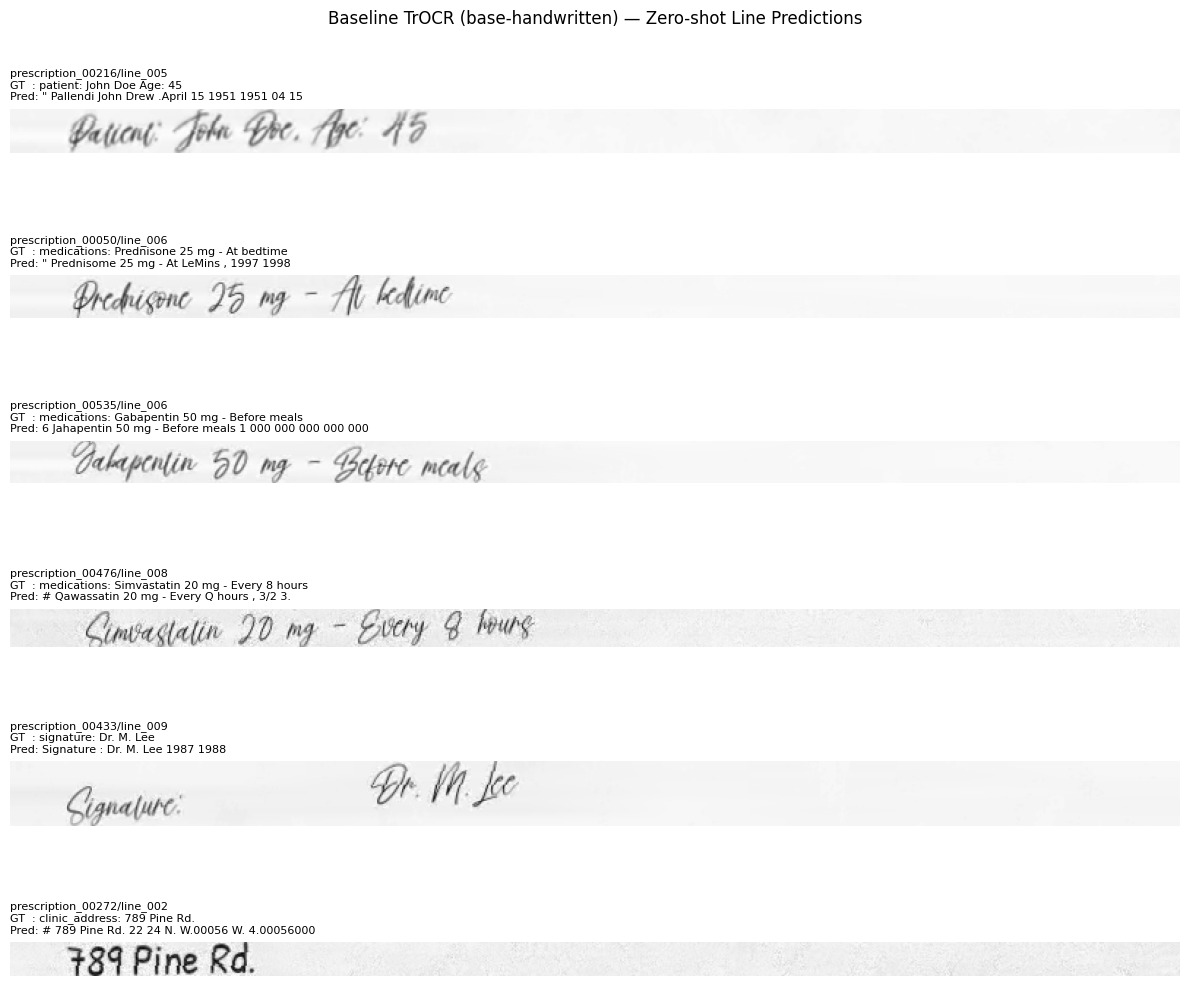
\includegraphics[width=0.8\textwidth]{pics/zero_shot_learning.jpg}
\caption{Baseline TrOCR (zero-shot) predictions. The model struggles with the domain-specific vocabulary and fails to output the targeted metadata structures, often resulting in severe hallucinations.}
\label{fig:zero_shot}
\end{figure}

Post fine-tuning, the model reliably captures both the raw text and the structured entity prefixes (e.g., \texttt{medications:}, \texttt{clinic\_name:}) required for downstream extraction (Figure \ref{fig:fine_tuned}).

\begin{figure}[H]
\centering
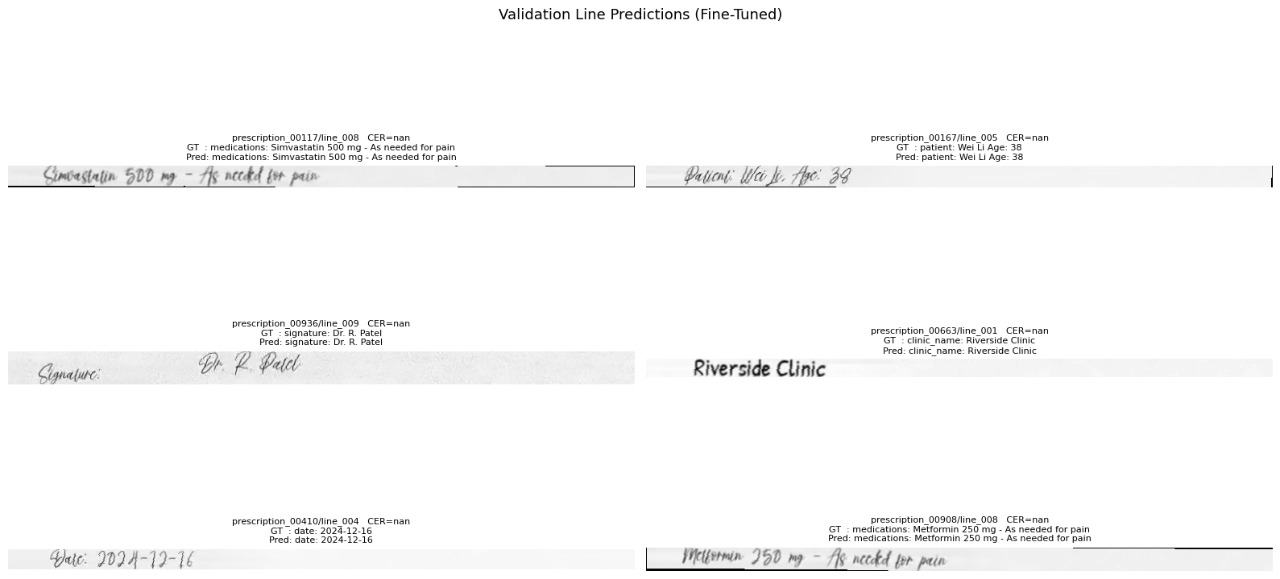
\includegraphics[width=\textwidth]{pics/after_learning.jpg}
\caption{Validation predictions after fine-tuning. The model successfully transcribes cursive handwriting and correctly formats the output into the expected structural schema.}
\label{fig:fine_tuned}
\end{figure}

\subsection{Failure Analysis}
The model still struggles on (a) tightly overlapping cursive strokes, (b) drug names rare in the training set, and (c) crops with strong shadows that survive preprocessing.

\clearpage
\newpage

\section{API and Frontend}
\label{sec:api}

\subsection{FastAPI Backend}
The backend lives in \texttt{api/main.py}. It loads the OCR pipeline once at startup and exposes two endpoints:
\begin{itemize}[noitemsep, topsep=0pt]
    \item \texttt{GET /health} --- liveness probe, returns model-loaded status.
    \item \texttt{POST /predict} --- accepts a multipart image upload, returns the OCR JSON.
\end{itemize}

% IMAGE: Screenshot of the auto-generated FastAPI Swagger UI at /docs
% Source: run `make run-api`, open http://localhost:8000/docs in a browser, take a screenshot
\begin{figure}[H]
\centering
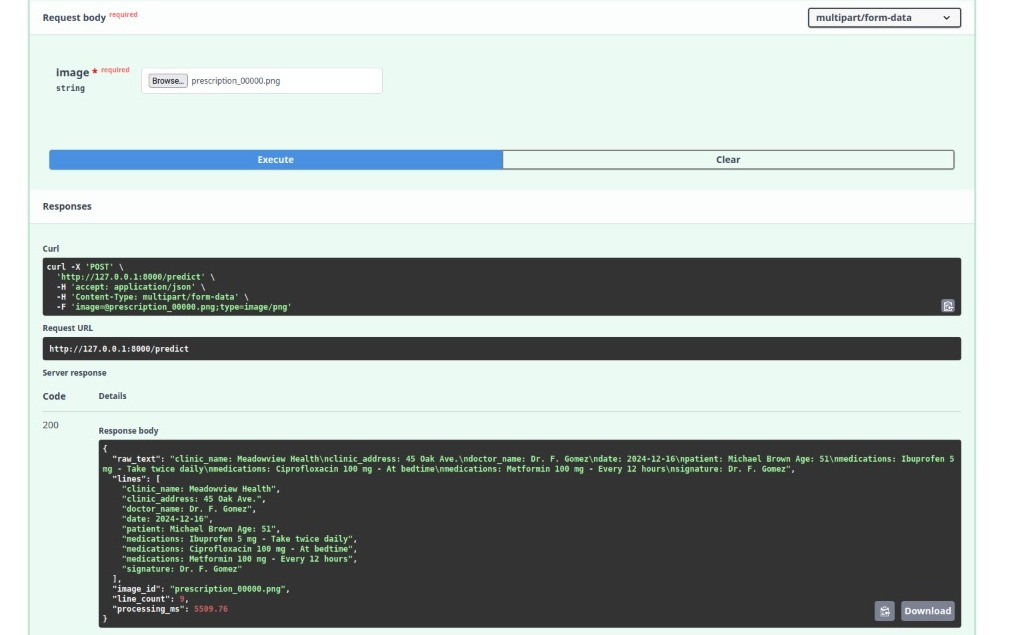
\includegraphics[width=0.9\textwidth]{pics/api_screen.jpg}
\caption{FastAPI auto-generated Swagger UI exposing \texttt{/health} and \texttt{/predict}.}
\label{fig:swagger}
\end{figure}
\clearpage
\newpage
\subsection{React + Vite Frontend}
The frontend (\texttt{frontend/}) is a Vite-powered React app that uploads an image to \texttt{/predict} and renders the predicted lines, total processing time, and raw text.

% IMAGE: Frontend after a prediction — image preview + extracted text
% Source: same dev server, upload a sample and screenshot the results state
\begin{figure}[H]
\centering
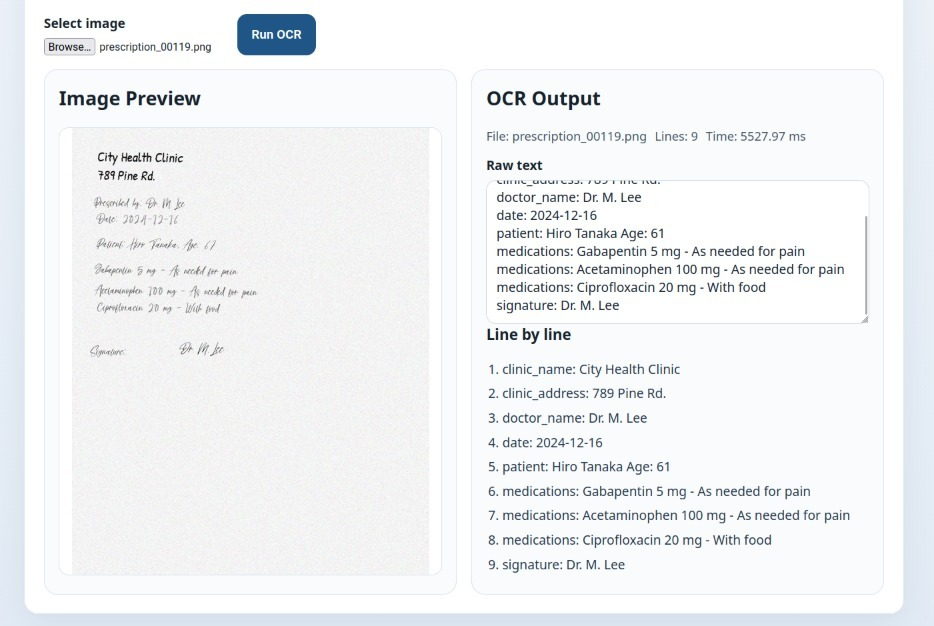
\includegraphics[width=0.85\textwidth]{pics/frontend_screen.jpg}
\caption{Prediction results view showing extracted lines and processing time.}
\end{figure}

\clearpage
\newpage

\section{Discussion and Limitations}

The fine-tuned model meaningfully outperforms zero-shot TrOCR on prescription-style handwriting, validating the choice of architecture and training recipe. Several limitations remain:
\begin{itemize}[noitemsep, topsep=0pt]
    \item \textbf{Dataset scale.} The public dataset is small relative to the variability of real prescriptions; performance on out-of-distribution handwriting drops.
    \item \textbf{Line segmentation as a separate stage.} Errors there cascade into TrOCR. A layout-aware model (Donut, LayoutLMv3) could remove the segmentation step entirely.
    \item \textbf{No formulary normalization.} Predicted drug names are not matched against a real drug database, so typos in the prediction are not corrected against a known vocabulary.
    \item \textbf{No multilingual support.} The current model is trained on English/Latin-script prescriptions only.
\end{itemize}

% IMAGE (optional): Future architecture sketch — e.g. layout-aware end-to-end model + formulary linker
% Source: design your own diagram, similar style to Figure 1
\begin{figure}[H]
\centering
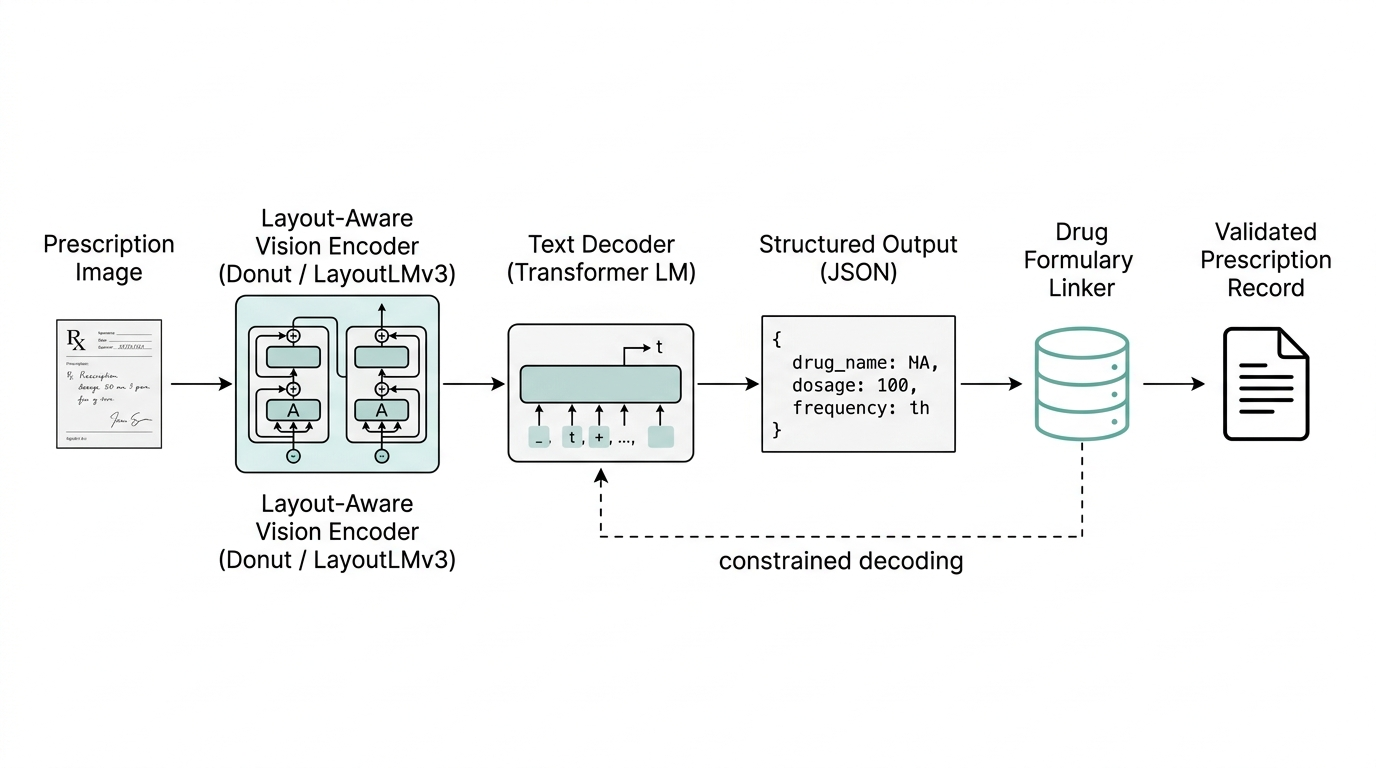
\includegraphics[width=1\textwidth]{pics/upgraded_architecture.png}
\caption{Sketch of a future end-to-end layout-aware OCR pipeline with drug-database normalization.}
\end{figure}

\clearpage
\newpage

\section{Technologies Used}

\subsection{PyTorch}
\begin{minipage}{0.7\textwidth}
PyTorch is the deep-learning framework underlying our entire training and inference stack. We used it for tensor operations, GPU acceleration during training, and model serialization.
\end{minipage}\hspace{.2in}
\begin{minipage}{0.25\textwidth}\centering
% LOGO: PyTorch | Source: https://pytorch.org/assets/images/pytorch-logo.png

\includegraphics[width=0.7\textwidth]{pics/tech/pytorch.png}
\end{minipage}

\vspace{.15in}

\subsection{HuggingFace Transformers}
\begin{minipage}{0.7\textwidth}
The Transformers library provides the \texttt{VisionEncoderDecoderModel} and \texttt{TrOCRProcessor} classes used throughout the project, plus the Hub integration for checkpoint sharing.
\end{minipage}\hspace{.2in}
\begin{minipage}{0.25\textwidth}\centering

\includegraphics[width=0.7\textwidth]{pics/tech/hugging_face.jpg}
\end{minipage}

\vspace{.15in}

\subsection{FastAPI}
\begin{minipage}{0.7\textwidth}
FastAPI serves the OCR pipeline over HTTP. It auto-generates Swagger documentation, supports asynchronous request handling, and integrates cleanly with Pydantic schemas.
\end{minipage}\hspace{.2in}
\begin{minipage}{0.25\textwidth}\centering
% LOGO: FastAPI | Source: https://fastapi.tiangolo.com/img/logo-margin/logo-teal.png

\includegraphics[width=0.5\textwidth]{pics/tech/fastapi.png}
\end{minipage}

\vspace{.15in}

\subsection{React + Vite}
\begin{minipage}{0.7\textwidth}
The frontend is a single-page React application bundled with Vite. It provides image upload, a live preview, and renders the OCR JSON returned by the API.
\end{minipage}\hspace{.2in}
\begin{minipage}{0.25\textwidth}\centering
% LOGO: React | Source: https://react.dev/favicon.ico (or official logo from reactjs.org/logo)

\includegraphics[width=0.55\textwidth]{pics/tech/react.png}
\end{minipage}

\vspace{.15in}

\subsection{Docker}
\begin{minipage}{0.75\textwidth}
The whole API is shipped as a Docker image so the deployment environment is reproducible across machines.
\end{minipage}\hspace{.2in}
\begin{minipage}{0.25\textwidth}\centering
% LOGO: Docker | Source: https://www.docker.com/wp-content/uploads/2022/03/Moby-logo.png

\includegraphics[width=0.7\textwidth]{pics/tech/docker.png}
\end{minipage}

\vspace{.15in}

\subsection{Kaggle}
\begin{minipage}{0.7\textwidth}
Kaggle's free 2$\times$T4 notebook environment hosted the fine-tuning runs. The notebook is automated end-to-end, from dataset download to Hub push.
\end{minipage}\hspace{.2in}
\begin{minipage}{0.25\textwidth}\centering
% LOGO: Kaggle | Source: https://www.kaggle.com/static/images/site-logo.svg

\includegraphics[width=0.7\textwidth]{pics/tech/kaggle.png}
\end{minipage}

\vspace{.15in}

\subsection{GitHub}
\begin{minipage}{0.7\textwidth}
GitHub hosts the source code and tracks history. Branches and pull requests structured the team workflow.
\end{minipage}\hspace{.2in}
\begin{minipage}{0.25\textwidth}\centering
% LOGO: GitHub | Source: https://github.com/logos

\includegraphics[width=0.6\textwidth]{pics/tech/github.png}
\end{minipage}

\clearpage
\newpage

\section{Conclusion}

This project shows that a fine-tuned vision encoder--decoder can transcribe handwritten medical prescriptions with practical accuracy, and that the resulting model can be wrapped in a clean API and a usable frontend. TrOCR's combination of a pretrained image encoder and a language-model decoder is well-matched to the noisy, vocabulary-specific nature of prescription text. The remaining gaps --- dataset scale, layout awareness, drug-name normalization --- point clearly at the next iteration: a larger, curated dataset; a layout-aware end-to-end model such as Donut or LayoutLMv3; and a post-OCR linker that grounds predictions against a real drug formulary.

\begin{thebibliography}{9}

\bibitem{trocr}
M.~Li, T.~Lv, J.~Chen, et al., \textit{TrOCR: Transformer-based Optical Character Recognition with Pre-trained Models}, arXiv:2109.10282, 2021.
\url{https://arxiv.org/abs/2109.10282}

\bibitem{vit}
A.~Dosovitskiy et al., \textit{An Image is Worth 16x16 Words: Transformers for Image Recognition at Scale}, ICLR, 2021.
\url{https://arxiv.org/abs/2010.11929}

\bibitem{beit}
H.~Bao, L.~Dong, S.~Piao, F.~Wei, \textit{BEiT: BERT Pre-Training of Image Transformers}, ICLR, 2022.
\url{https://arxiv.org/abs/2106.08254}

\bibitem{hf_transformers}
HuggingFace Transformers documentation. \url{https://huggingface.co/docs/transformers}

\bibitem{trocr_hf}
\textit{microsoft/trocr-base-handwritten} model card. \url{https://huggingface.co/microsoft/trocr-base-handwritten}

\bibitem{dataset}
\textit{chinmays18/medical-prescription-dataset}. \url{https://huggingface.co/datasets/chinmays18/medical-prescription-dataset}

\bibitem{fastapi}
S.~Ramirez, FastAPI documentation. \url{https://fastapi.tiangolo.com/}

\bibitem{donut}
G.~Kim et al., \textit{OCR-free Document Understanding Transformer (Donut)}, ECCV, 2022. \url{https://arxiv.org/abs/2111.15664}

\end{thebibliography}

\end{document}
